\documentclass[10pt,a4paper,twocolumn]{article}
\usepackage[margin=1.7cm]{geometry}
\usepackage[T1]{fontenc}
\usepackage{lmodern,microtype,amsmath,booktabs,graphicx}
\usepackage[table]{xcolor}
\usepackage{tikz}
\usetikzlibrary{arrows.meta,positioning}
\usepackage[colorlinks=true,urlcolor=blue,citecolor=blue]{hyperref}
\definecolor{navy}{HTML}{132C45}
\newcommand{\na}{\textcolor{red}{pending}}
% ----- RESULTS-BEGIN
% Populated only by eval.paper_numbers after the hardened run.
% ----- RESULTS-END
\title{\color{navy}CASSANDRA / AURORA\\Hardened Implementation and Evaluation Report}
\author{\small Youssef Mhamdi, Mayssam Hergli, Rami Troudi, Eya Jendoubi, Youssef Atig\\
\small National Institute of Applied Sciences and Technology (INSAT), Tunis, Tunisia\\
\small\texttt{rami.troudi@insat.ucar.tn}}
\date{Hardened research demonstrator --- 12 October 2026}
\begin{document}
\maketitle
\begin{abstract}
CASSANDRA studies whether correlated cyber and physical evidence can provide useful warning before a satellite reaches an operational critical state, and support a proportionate defensive response. The implemented AURORA demonstrator combines a custom 12-satellite synthetic twin, an MQTT integration bus, a temporal graph forecasting ensemble, an observation-seeded counterfactual sandbox, and a safety-gated runtime with recovery verification. This revision corrects noncausal feature initialization, adds observation freshness, aligns failure criteria across prediction and response, restricts actions to their implemented effects, and treats unavailable uncertainty conservatively. Fresh preliminary forecast measurements are reported; full runtime-policy evaluation remains pending. Synthetic performance, including replay of OPS-SAT noise, is not flight attack validation. The ESP8266 endpoint exercises software and hardware interfaces with emulated temperature; physical thermal recovery and embedded-target performance remain unverified.
\end{abstract}
\noindent\textbf{Keywords:} satellite cybersecurity, early warning, cyber-physical resilience, temporal graph forecasting, counterfactual response.

\section{Context and problem}
Spacecraft subsystems are coupled: an unauthorized command can change actuation, thermal load, power consumption and attitude before a single critical limit is reached. A present-state alarm answers whether a value is abnormal; early warning asks whether observations imply an approaching operational failure. SPARTA supplies a vocabulary for attack and countermeasure relations~\cite{sparta}, while engineering dependencies constrain which effects are plausible.

For synthetic satellite $s$, this study defines
\begin{equation}
 F_s = (T_s>45\,^{\circ}\mathrm{C})\lor(\mathrm{SOC}_s<30\%)\lor(|\theta_s|>10^{\circ}).
\end{equation}
These are study limits, not universal spacecraft requirements. The learned task is to estimate $P(F_s<t+\Delta\mid\mathcal O_{\leq t})$ at horizons $\Delta\in\{10,30,60,120\}$ seconds. A useful response must reduce residual risk while preserving service and avoid unsafe decisions when observations or uncertainty estimates are incomplete.

\section{Implemented architecture}
\begin{figure}[ht]
\centering
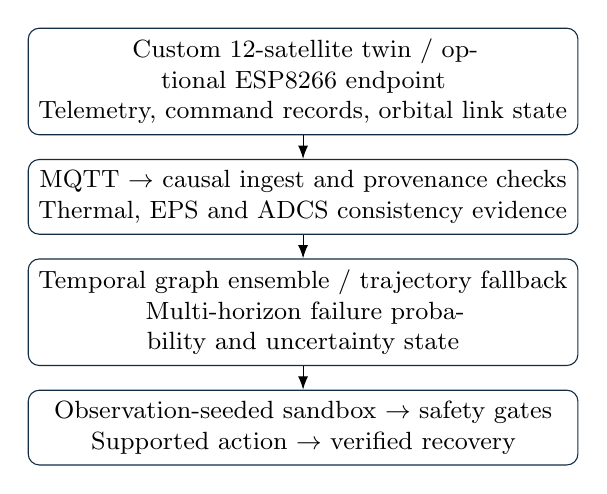
\begin{tikzpicture}[node distance=3mm, every node/.style={draw=navy,rounded corners,align=center,font=\small,text width=6.7cm,inner sep=4pt}, >={Latex}]
\node (a) {Custom 12-satellite twin / optional ESP8266 endpoint\\Telemetry, command records, orbital link state};
\node[below=of a] (b) {MQTT $\rightarrow$ causal ingest and provenance checks\\Thermal, EPS and ADCS consistency evidence};
\node[below=of b] (c) {Temporal graph ensemble / trajectory fallback\\Multi-horizon failure probability and uncertainty state};
\node[below=of c] (d) {Observation-seeded sandbox $\rightarrow$ safety gates\\Supported action $\rightarrow$ verified recovery};
\draw[->] (a)--(b);\draw[->] (b)--(c);\draw[->] (c)--(d);
\end{tikzpicture}
\caption{Implemented pipeline. Response commands return through MQTT; the dashboard displays observations, forecasts and decision evidence. Ground truth is excluded from runtime inputs.}
\end{figure}

Each satellite has six subsystem nodes and an aggregation node. A 30-second observation window is encoded by GRUs, followed by typed graph message passing over engineering relations, SPARTA annotations and currently enabled inter-satellite links. Learned coupling statistics and engineering residual features supplement the temporal representation. This implementation is a windowed temporal graph model; it does not claim equivalence to an event-memory TGN architecture.

The full protocol specifies five models with distinct training seeds; the deadline-bounded submission uses the two completed members. Temperature scaling uses validation data. Ensemble spread is reported as standard deviation, not variance; it is an imperfect uncertainty signal rather than a guarantee of calibrated epistemic uncertainty~\cite{ensemble,calibration}.

\subsection{Causal and trusted observations}
Offline training and live inference share a single event-to-frame implementation. Events take effect on arrival; older or duplicate subsystem timestamps cannot overwrite newer values. Unseen channels begin at zero, accompanied by missing-sample indicators and capped ages for temperature, SOC and attitude. Values are held forward only. The resulting input has 33 channels per satellite, replacing the earlier 27-channel representation. Regression tests include initial gaps, delayed and out-of-order messages, dropouts and offline/online equality.

The ingest stage retains source-mismatched messages as low-assurance evidence without replacing trusted observations. This enforces the configured source policy; a publisher-controlled source field alone provides no authentication. EPS power inconsistency and ADCS sensor-range checks complement the thermal freeze/heater monitor. Their events require corroboration and do not establish malicious intent.

\subsection{Response and recovery}
The sandbox starts from observed thermal, power, attitude and wheel state, with no future attacker queue. Its crossing checks use every enabled term of $F_s$. Candidate scoring is
\begin{equation}
 J(a)=w_rR(a)+w_m[1-U(a)]+w_cC(a).
\end{equation}
Here $R$ is residual risk, $U$ retained service and $C$ configured operational cost. Pre-action uncertainty is identical across candidates, so it is used by safety gates rather than added as a constant ranking term.

The implemented actions are no action, heater off (\texttt{cut\_heater}), local safe mode, blocking an observed ISL source, and budgeted quarantine. Heater off is not represented as generic subsystem repair. Unknown or invalid uncertainty has state \texttt{UNKNOWN}; high spread is \texttt{KNOWN\_HIGH}. Both withhold link isolation and quarantine, while allowing supported local protective actions and requesting ground review. Recovery requires present, safe evidence for all enabled failure dimensions and the existing persistence/thermal-calm conditions. Command execution is simulated at tick cadence; hardware actuation latency is not established here.

\section{Methodology}
The standard episode splits contain 800 training, 200 validation, 300 synthetic ID test, 300 held-out-family OOD test and 200 synthetic episodes with OPS-SAT residual noise and gaps. Complete episodes are separated between splits. The last split remains synthetic attack-to-failure evaluation: OPS-SAT contributes a noise/gap process, not a flight attack trajectory or flight failure labels~\cite{opssat}.

At a 60-second primary horizon, each method selects a validation threshold targeting 0.1\% benign-timestep false positives. Thresholds are applied unchanged to tests; the realized test false-positive rate can differ. Lead time is $T_{\rm critical}-T_{\rm alert}$ for detected failures; pre-onset alerts are counted separately. Evaluation every two seconds limits alert-time resolution to one second. Confidence intervals resample complete episodes.

The full planned comparison includes static limits, the trajectory predictor, LSTM autoencoder and GDN-style baseline. Planned ablations remove engineering relations, residual features, SPARTA relations, learned couplings, message passing, or command evidence; an unconstrained graph is also specified. Saturating recall alone cannot establish a contribution from graph structure.

A separate 48-episode hard set pairs attack and benign cases using the same seed, ground command origins and diagnostic bursts, with bounded benign heater, wheel-test or science operations. It reduces simple origin/precursor cues; its physically generated benign and malicious effects are still distinguishable and do not constitute adversarially indistinguishable classes. It is held out from training and threshold selection.

The implemented, pending paired runtime campaign uses the actual core, including persistence, gates, planning, escalation and recovery. Each defended run is paired with an undefended run using the same seed. A mismatch arm changes plant thermal capacity by $-20\%$ and conductance by $-30\%$, while keeping the sandbox nominal. This is a limited sensitivity study, not validation against an independent plant. The older simulator-snapshot evaluator is retained only as a legacy reference.

Adversarial evaluation applies bounded iterative perturbations to forgeable physical telemetry, excluding independent timing/missingness, heater-state and ground command evidence. The planned type-stratified sample and episode bootstrap intervals accompany recall and lead time. This evaluates the stated perturbation objective and budget, not all attacker capabilities.

\section{Implementation map and reproduction}
\begin{description}
\item[Observation path.] \texttt{ml/frames.py} is the shared event-to-frame builder; \texttt{cassandra/ingest.py} closes causal runtime ticks and enforces the configured source policy.
\item[Failure criteria.] \texttt{aurora\_common/criticality.py} provides the shared thermal, SOC and absolute-attitude checks used by the generator, recorder, planner and verifier.
\item[Safety and actions.] \texttt{cassandra/actions.py} records targets, prerequisites, effects, rollback/verification expectations and permissions under unknown uncertainty. \texttt{act.py} applies the policy.
\item[Evaluation.] \texttt{eval/harness.py} scores forecast operating points. \texttt{eval/runtime\_policy.py} runs paired real-core simulations. \texttt{hard\_benchmark.py} creates held-out matched-origin episodes; \texttt{robustness.py} reports stratified perturbation results and intervals.
\item[Provenance.] \texttt{scripts/freeze\_results.py} freezes result JSON, actual versions, successful command records, source/config/model digests and the dataset inventory. Rebuild the frozen record only after all stages succeed.
\end{description}

Checkpoints must carry the \texttt{causal-v2} schema and the exact 33-channel list. Older 27-channel releases are rejected; retraining is required. Cache output is published atomically. Training subprocess failures terminate the training orchestrator instead of silently producing an incomplete ensemble.

The pinned environment is Python 3.11 with \texttt{requirements.lock}. Project packaging explicitly includes runtime packages, MQTT dependency and bundled YAML. The fake-board broker test is a software interface test. A physical board, sensor and actuator must be tested separately before any hardware safety claim.

\section{Results}
% RESULTS-NARRATIVE-BEGIN
\textbf{Preliminary submission run.} The submission deadline limited this revision to two independently trained ensemble members (seeds 0 and 1), each trained with the unchanged eight-epoch configuration on 800 training episodes. The planned five-seed ensemble and seven ablations are not reported as completed. Temperature scaling and a target 0.1\% benign-step threshold used a separate 24-episode validation subset (the first eight indexed episodes of each kind); the realized validation FPR was 0.105\%. The resulting temperature was 0.662 and the ensemble alert threshold was 0.00846.

Standard test subsets likewise use the first eight indexed episodes of each kind; the matched hard set uses all 48 episodes. These are preliminary subset measurements, not full-split results. Scores are computed every 20 seconds and held forward, so lead-time resolution is up to 19 seconds. The planned two-second protocol remains the full-campaign configuration. Detection counts below refer to failing satellite cases, not independent episodes.

\begin{table}[ht]
\centering\footnotesize\setlength{\tabcolsep}{3pt}
\begin{tabular}{lrrrr}
\toprule
Set & Episodes & Hits/Failures & Lead (s) & FPR (\%)\\
\midrule
ID subset & 24 & 12/12 & 117.0 & 0.123 \\
OOD subset & 24 & 9/10 & 117.0 & 0.052 \\
Matched hard set & 48 & 24/24 & 134.5 & 0.093 \\
\bottomrule
\end{tabular}
\caption{Two-seed ensemble, 60-second forecast head, validation-selected threshold. Lead is the median among detected cases; FPR counts benign satellite-timesteps.}
\end{table}

For the ID, OOD and hard sets respectively, static-limit recall was 75.0\%, 40.0\% and 83.3\%; trajectory-baseline recall was 100\%, 70.0\% and 95.8\%. Their detected-case median leads were 83/80/74 seconds (static) and 16/14/12 seconds (trajectory). Every comparator used its own threshold selected on the same validation subset and the same scoring schedule. These comparisons do not isolate the effect of graph components.

Episode bootstrap (1,000 resamples) gave an OOD recall interval of 62.5--100\% and a median-lead interval of 80.5--126 seconds. ID and hard-set bootstrap recall intervals collapse at 100\% because no observed failures were missed; this does not establish perfect population recall. The corresponding median-lead intervals were 114--125.5 and 108--217 seconds. One, three and one pre-onset alarm events occurred across all satellites in the respective attack subsets; these are excluded from credited warning lead. A low validation-selected threshold can alert more than 60 seconds before failure and is not an autonomous-action authorization.

The full hardened software suite previously passed 196 tests, including MQTT software integration; additional focused regressions passed. The final expanded suite is recorded in the submission verification artifact. Completed model checkpoints and exact subset indices accompany the measurements. On this x86\_64 workstation, 50 inference repetitions for the two-model ensemble at one thread yielded 19.4 ms median and 21.6 ms p95; planning is excluded, so this does not establish embedded end-to-end timing. No completed full runtime-policy campaign, PGD robustness result, ablation result or OPS-SAT-noise test performance is claimed in this submission. Those evaluations remain next steps.
% RESULTS-NARRATIVE-END

\section{Prototype evidence and limitations}
The historical Phase-2 setup connects an ESP8266 emulated thermal endpoint through serial and Redis; the integrated implementation uses MQTT, a custom twin and a single-page dashboard. The supplied manuscript reports a 2.3-second alert and a roughly 4.5-second margin before its counterfactual limit; the demo note reports approximately 6 seconds for the alert. No raw log sufficient to reconcile those values was supplied. This revision therefore does not reuse them as reproduced performance measurements.

Software broker tests and the fake-board bridge can verify integration and command/state transitions. They cannot validate a real heater, sensor calibration, physical thermal time constants or flight actuation. No Raspberry Pi inference/planning timing, native NOS3/cFS integration, ESA-ADB mission test, or physical multi-node ESP32 demonstration is claimed. CuCD-ID audit and SCAD propagation analysis are separate dataset roles, not proof of this forecaster's failure-warning performance.

Further limitations include generator-specific dynamics, imperfectly independent channels, shared simulator/model structure, heuristic consistency thresholds, uncalibrated action costs, incomplete attack observability and untested distribution shifts. A single destructive command without an observable precursor may provide no warning interval. Correct recovery logic cannot guarantee recovery from an unsupported physical fault.

\section{Conclusion and next steps}
CASSANDRA is an integrated research demonstrator for causal multi-domain warning and constrained defensive response. The hardened implementation makes observation timing, failure criteria, supported actions and uncertainty handling explicit. The evidence should be read at three separate levels: synthetic forecast performance, complete software-policy outcomes, and interface-level hardware emulation. Next steps are independent-plant testing, broader matched benign operations, physical sensor/actuator calibration, embedded latency measurement and operational telemetry transfer tests. Claims of flight readiness or a general graph-model advantage require additional evidence.

\begin{thebibliography}{9}
\bibitem{sparta} The Aerospace Corporation, ``SPARTA: Space Attack Research and Tactic Analysis,'' \url{https://sparta.aerospace.org/}.
\bibitem{opssat} B. Ruszczak, K. Kotowski, D. Evans and J. Nalepa, ``The OPS-SAT benchmark for detecting anomalies in satellite telemetry,'' \emph{Scientific Data}, vol. 12, art. 710, 2025.
\bibitem{ensemble} B. Lakshminarayanan, A. Pritzel and C. Blundell, ``Simple and scalable predictive uncertainty estimation using deep ensembles,'' \emph{NeurIPS}, 2017.
\bibitem{calibration} C. Guo, G. Pleiss, Y. Sun and K. Q. Weinberger, ``On calibration of modern neural networks,'' \emph{ICML}, 2017.
\bibitem{repo} CASSANDRA/AURORA, hardened implementation, branch \texttt{rami}; preliminary reproducibility record: \texttt{results/submission/manifest.json}.
\end{thebibliography}
\end{document}
